% Slides accompanying "Learn RISC-V CPU Implementation and BSV" book
% Copyright (c) 2024 Rishiyur S. Nikhil, All Rights Reserved

% -*- mode: fundamental -*-

% Slides accompanying "Learn RISC-V CPU Implementation and BSV" book
% Copyright (c) 2024 Rishiyur S. Nikhil, All Rights Reserved

% This is a preamble shared by all the slide decks

\documentclass[10pt, aspectratio=169]{beamer}

% \documentclass[17pt]{beamer}

% Avail. font sizes: 8pt, 9pt, 10pt, 11pt, 12pt, 14pt, 17pt, 20pt.
% Default font size is 11pt (= 22pt in full screen mode).

\usepackage{verbatim}
\usepackage{fancyvrb}
\usepackage{listings}

% ================================================================
% Themes

\usetheme{Madrid}          % Line at bottom: Author (affiliation), OptTitle, Conf, page 

% \usetheme{Copenhagen}    % Same as Madrid except bottom line: Author, OptTitle

% \usetheme{Berkeley}    % Takes up 1-inch border on left and top

% ----------------
% colorthemes
% (default), beaver, beetle, seahorse, wolverine

\usecolortheme{seahorse}

% ================================================================
% Customization: show table of contents before each section
% Use \AtBeginSubsection    to show before each subsection

% \AtBeginSection[]
% {
%   \begin{frame}
%     \frametitle{Table of Contents}
%     \tableofcontents[currentsection]
%   \end{frame}
% }

% ================================================================

% ----------------
% The bsc compiler and BSV language
\newcommand{\bsc}{\emph{bsc}}
\newcommand{\BSV}{\bf{BSV}}
% ----------------
% ITALICISE WORDS
\newcommand{\ie}{\emph{i.e.,}}
\newcommand{\eg}{\emph{e.g.,}}
\newcommand{\Eg}{\emph{E.g.,}}
\newcommand{\etc}{\emph{etc.}}
\newcommand{\via}{\emph{via}}
\newcommand{\vs}{\emph{vs.}}

% ----------------
% EMPTY BOXES OF VARIOUS WIDTHS, FOR INDENTATION

\newcommand{\hm}{\hspace*{1em}}
\newcommand{\hmm}{\hspace*{2em}}
\newcommand{\hmmm}{\hspace*{3em}}
\newcommand{\hmmmm}{\hspace*{4em}}

% ----------------
% Convenient widths

\newlength{\hlessmm}
\setlength{\hlessmm}{\textwidth}
\addtolength{\hlessmm}{-2em}

\newlength{\hlessmmm}
\setlength{\hlessmmm}{\textwidth}
\addtolength{\hlessmmm}{-3em}

\newlength{\hlessmmmm}
\setlength{\hlessmmmm}{\textwidth}
\addtolength{\hlessmmmm}{-4em}

% ================================================================
% Title page

\title[Learn CPU design \& BSV]{Learn RISC-V CPU Implementation and BSV}

\subtitle{(BSV: a High-Level Hardware Design Language)}

\author[{\copyright} R.S.Nikhil]{Rishiyur S.~Nikhil}
% \institute{Bluespec, Inc.}

% Date is set differently in each slide deck

% \logo{
\includegraphics[height=0.6cm]{../Figures/Bluespec_Logo_2022-10}}

% End of preamble
% ****************************************************************


\date{L14: RISC-V: The Drum CPU, using Rules}

% ****************************************************************

\begin{document}

% ================================================================

\begin{frame}
 \titlepage

 \begin{center}
  
\includegraphics[height=1cm]{Bluespec_Logo_2022-10}
 \end{center}

\end{frame}

% ================================================================

% -*- mode: fundamental -*-

% ================================================================

\begin{frame}[fragile]
\frametitle{Reminders}

\footnotesize

Please git clone: \url{https://github.com/rsnikhil/Learn_Bluespec_and_RISCV_Design} \\
(git pull for latest version).  Repsitory structure:

\vspace{1ex}

\begin{minipage}{0.5\textwidth}\scriptsize
\begin{Verbatim}[frame=single, numbers=left]
    ./Book_BLang_RISCV.pdf
      Slides/
          Slides_01_Intro.pdf
          Slides_02_ISA.pdf
          ...
      Exercises/
          Ex-03-A-Hello-World/
          Ex-03-B-Top-and-DUT/
          ...
      Code/
          src_Top/
          src_Drum/
          src_Fife/
          src_Common/
          ...
      Doc/Installing_bsc_Verilator_etc.{adoc,html}
\end{Verbatim}
\end{minipage}
\hm
\begin{minipage}{0.45\textwidth}
\begin{itemize}

 \item Slides and Exercise are numbered in sync with book Chapter numbers.

 \item For Exercises, please see Appendix E of the book.  Some (not
       all) exercises have associated code in the {\tt Exercises/}
       directory.

\end{itemize}
\end{minipage}

\vspace{2ex}

To compile and run the code for exercises, Drum and Fife, please make sure you have installed:

\begin{itemize}

 \item \emph{bsc} compiler (see \url{https://github.com/B-Lang-org/bsc})

 \item Verilator compiler (see \url{https://www.verilator.org/})
\end{itemize}

\footnotesize

\end{frame}

% ================================================================

\begin{frame}
\frametitle{Chapter Roadmap}

\footnotesize

\begin{center}
\frame{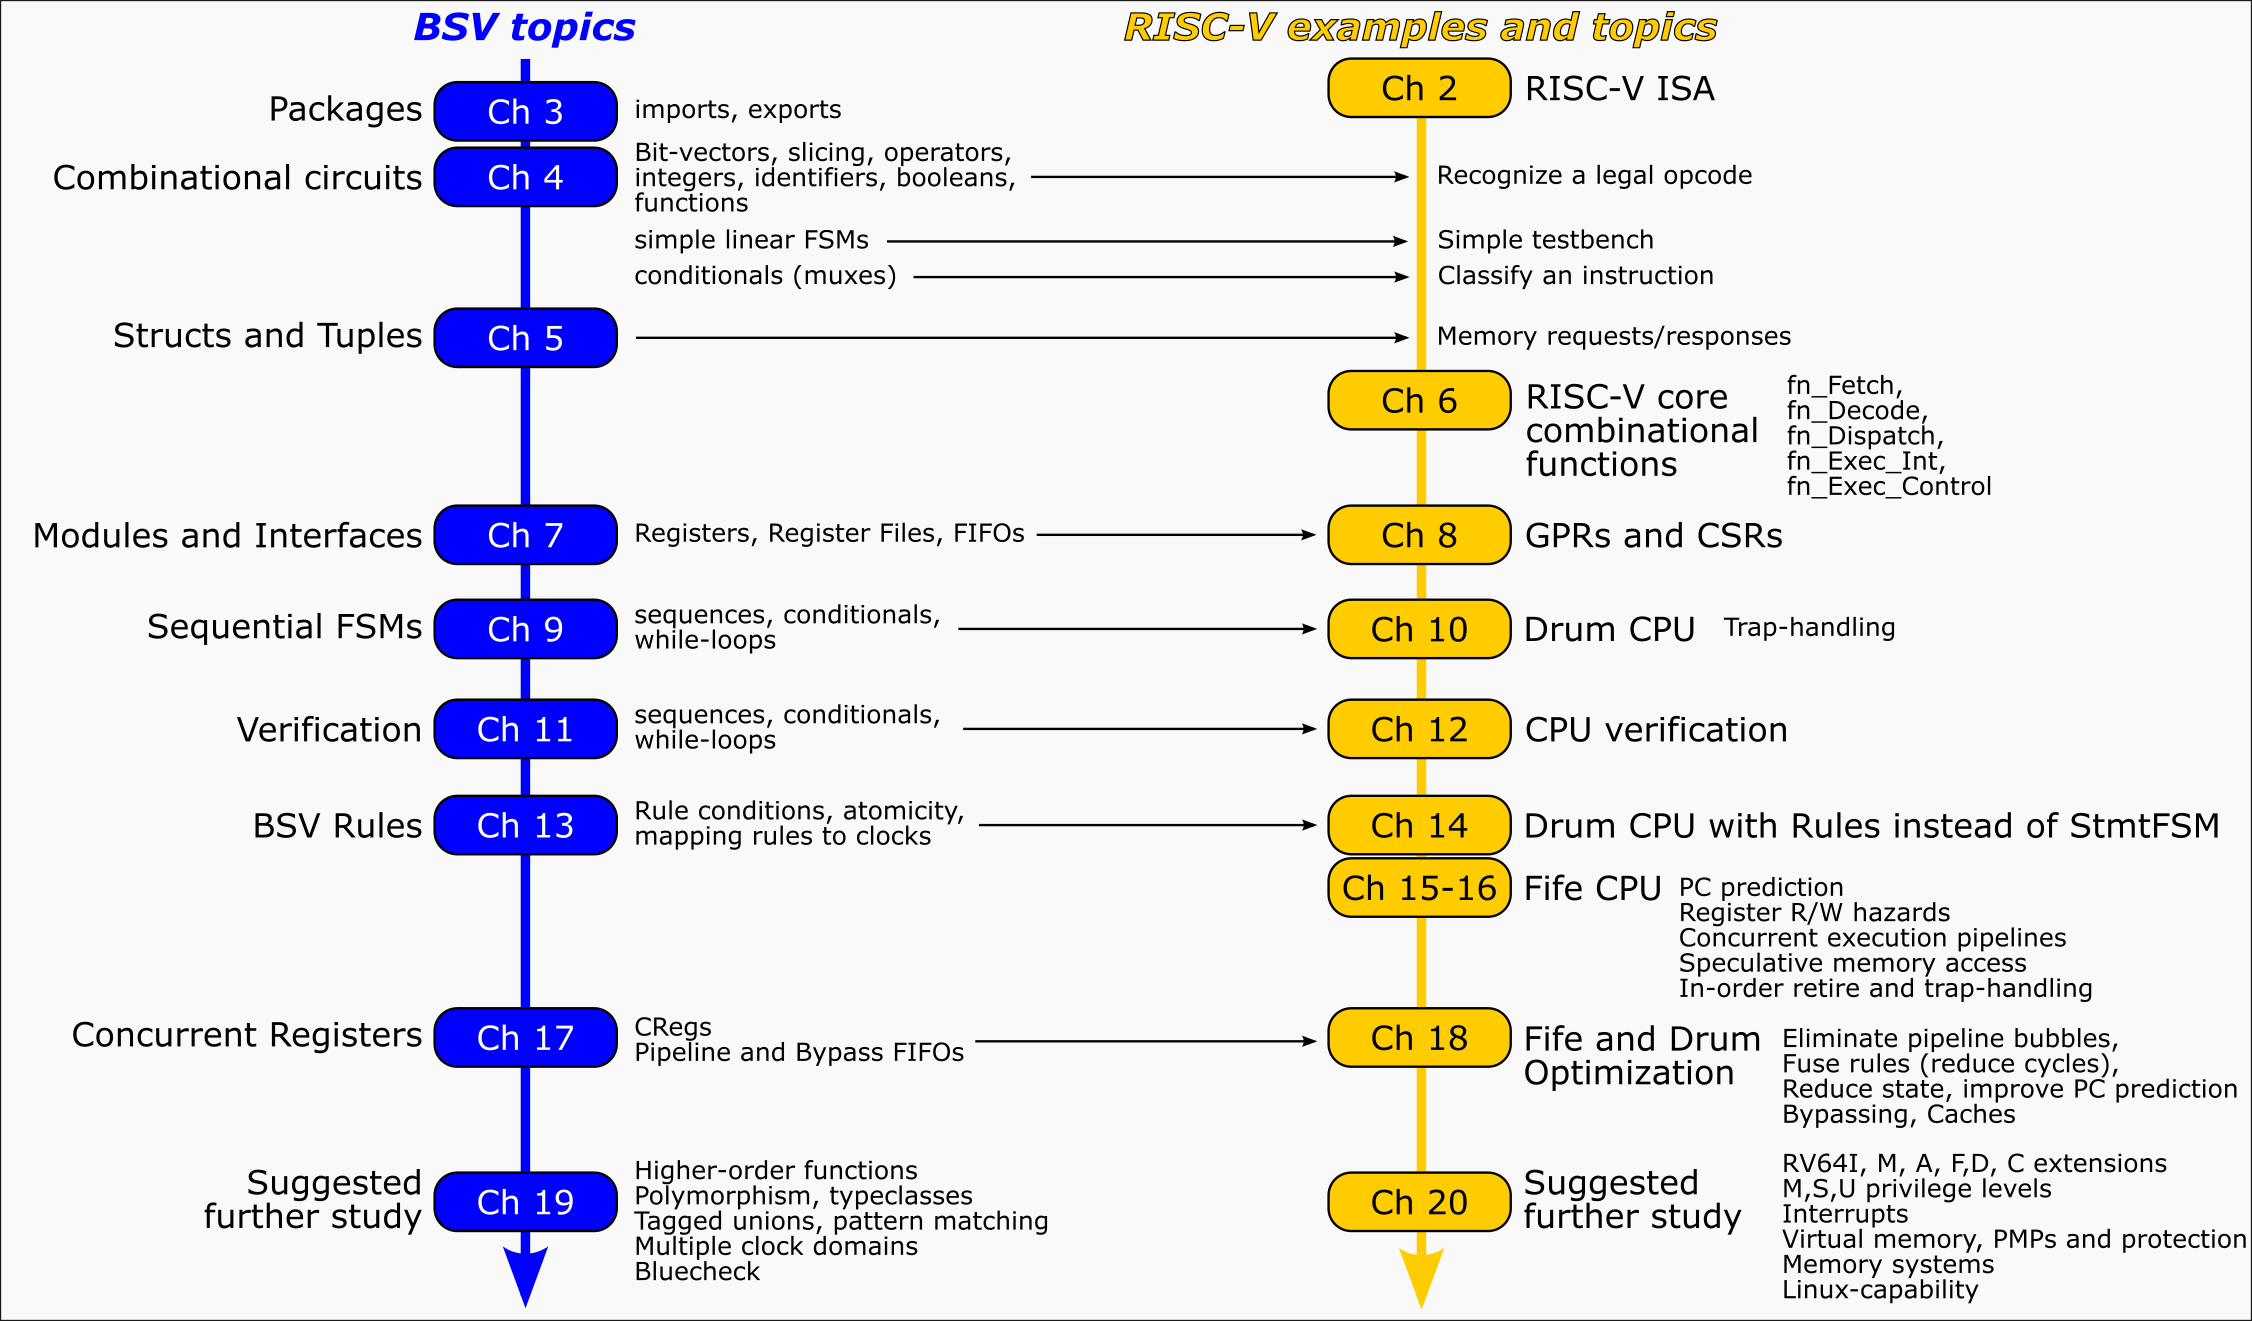
\includegraphics[height=0.825\textheight]{Fig_Chapter_Roadmap}}
\end{center}

\end{frame}

% ================================================================


% ================================================================

\begin{frame}
\frametitle{Flow of information between stages in Drum and Fife}

\footnotesize

\begin{center}
 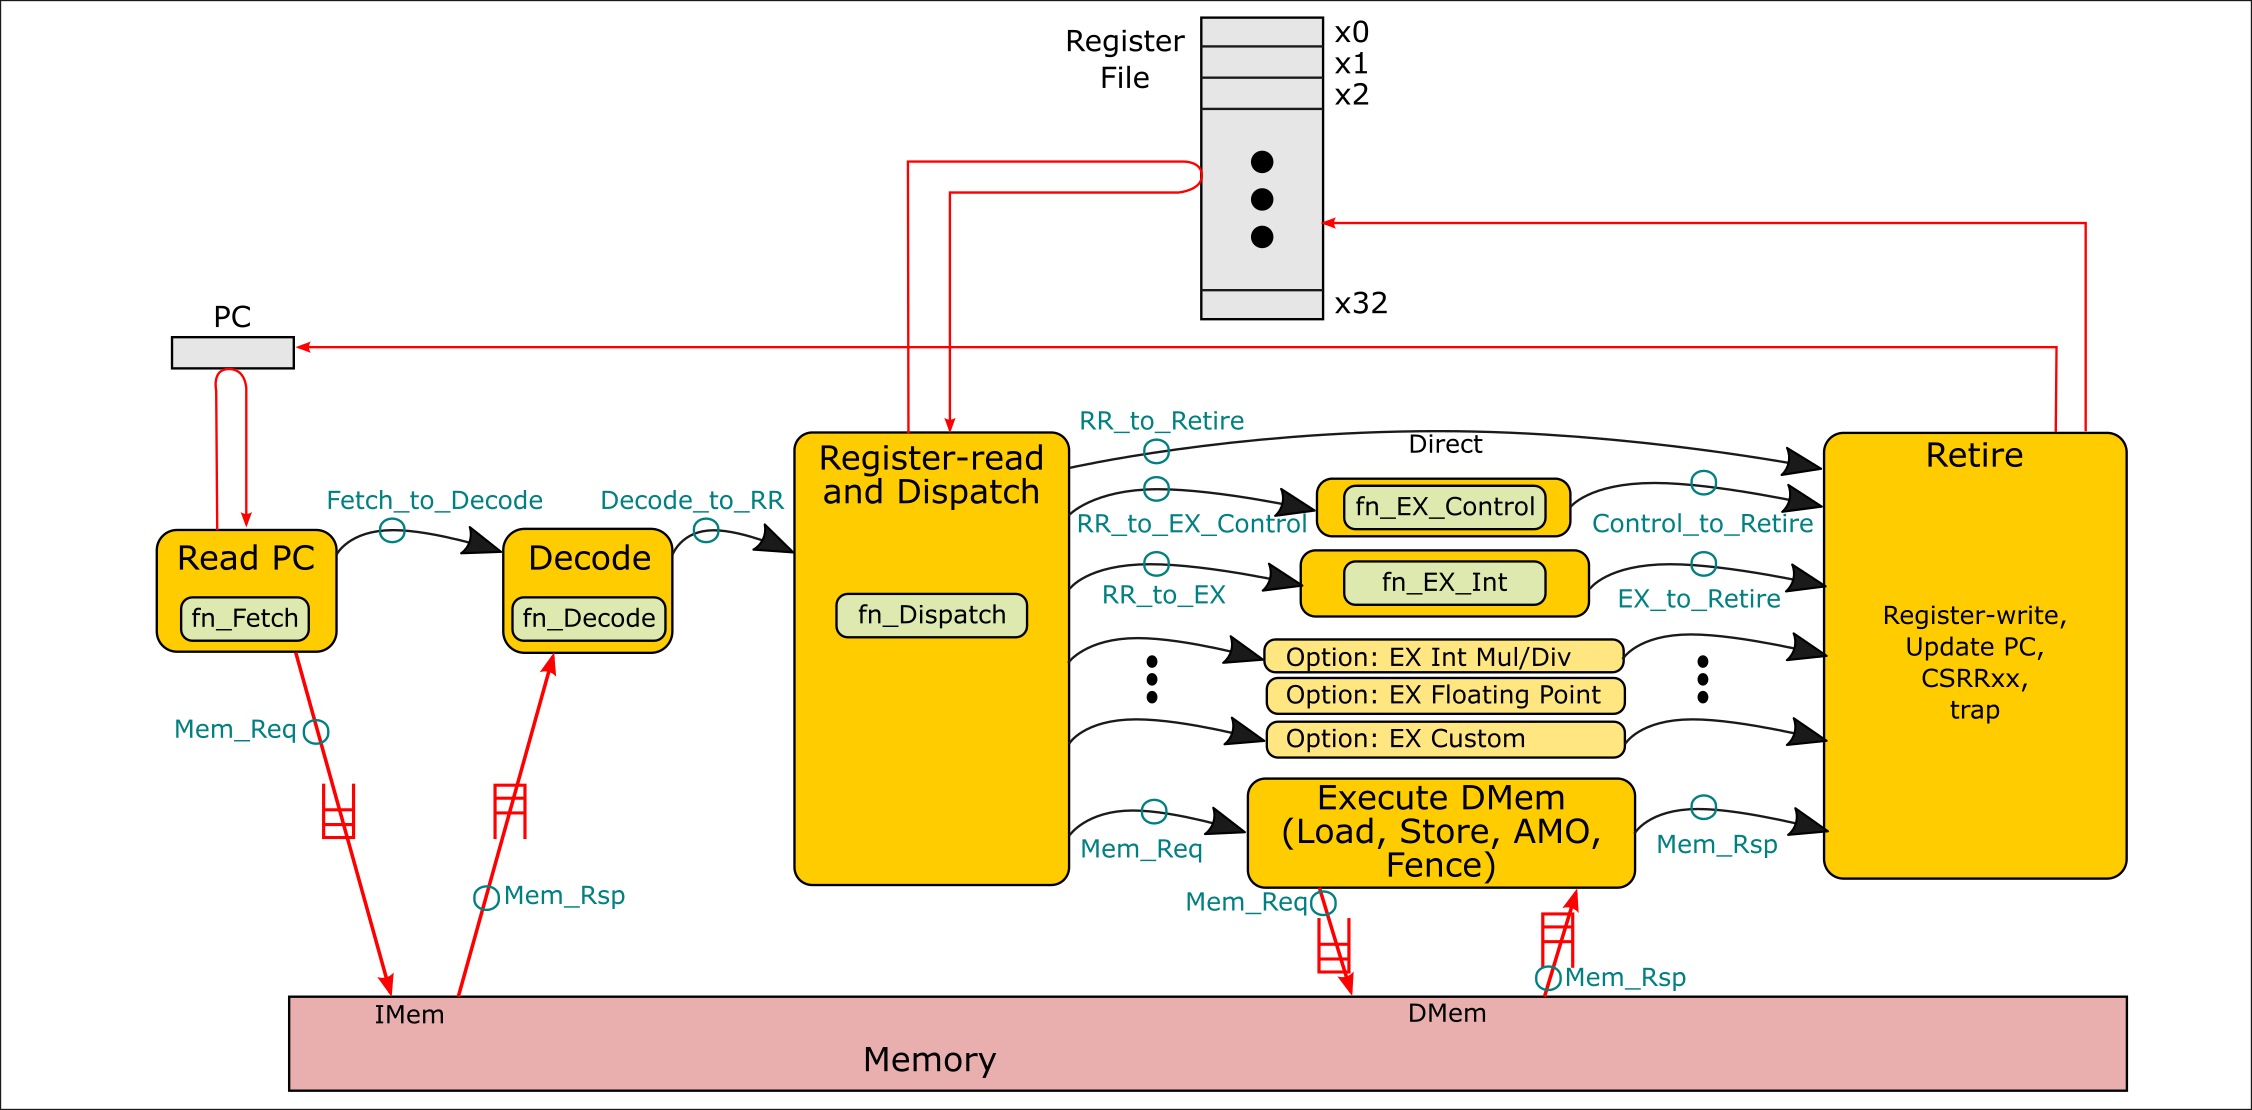
\includegraphics[height=0.6\textheight]{Fig_Instr_Exec_w_structs}
\end{center}

\end{frame}

% ================================================================

\begin{frame}
\frametitle{Table of Contents}

\tableofcontents

\end{frame}

% ****************************************************************

\section{The Drum CPU, using Rules}

\begin{frame}

\begin{center}
  {\LARGE RISC-V: The Drum CPU, using Rules instead of {\tt StmtFSM}}
\end{center}

\end{frame}

% ================================================================

\begin{frame}[fragile]
\frametitle{The Drum CPU, using Rules instead of {\tt StmtFSM}}

\footnotesize

This is a short chapter demonstrating a manual translation of the Drum
CPU module from one using {\tt StmtFSM} to one using Rules instead.

\vxx

This reinforces our claim that {\tt StmtFSM} does not add any new
semantics to {\BSV}; it is simply a higher-level notation that can be
used fruitfully in certain circumstances (``structured processes'').

\vxx

Please examine the source files in {\tt src\_Drum/} directory:

\begin{center}
\mbox{{\tt CPU.bsv} \hmm {\tt Drum\_FSM.bsv} \hmm {\tt Drum\_Rules.bsv}}
\end{center}

{\tt CPU.bsv} is the common file; it ``includes'' either {\tt
Drum\_FSM.bsv} ({\tt StmtFSM} version) or {\tt Drum\_Rules.bsv} (Rules
version).

By examining the latter two files side by side, we can observe the
equivalence.  Briefly:

\begin{itemize}

  \item We define an ``{\tt enum}'' type that gives a symbolic name to
      each action-step in the FSM, and introduce a ``sequencer''
      register to hold a value of this type.

  \item We convert each action in the FSM to a rule

      \begin{itemize}\footnotesize

        \item whose rule-condition allows it to execute only when the
            sequencer says it is its turn to execute, and

        \item whose rule-body ``increments'' the sequencer to the next FSM step.
      \end{itemize}

\end{itemize}

\end{frame}

% ================================================================

\begin{frame}[fragile]
\frametitle{Advantages of the Rules version}

\footnotesize

{\tt StmtFSM} only permits \emph{structured} process composition,
{\ie} properly nested sequencing, if-then-else, while-loops.

\vxxxx

The Rules version makes it easy to depart from such properly nested
structure and ``short-circuit'' certain flows for better performance.

\vxx

For example:
\begin{itemize}

  \item If we detect an exception in rule {\tt rl\_Decode} (and,
      indeed, in any of the other rules), we can immediatelly handle
      the exception and ``jump'' back to the Fetch step, thereby
      saving several cycles.

  \item In {\tt rl\_EX\_Control} and {\tt rl\_EX\_Int}, if there is no
      exception, we can immmediately perform any register write and
      ``jump'' back to the Fetch rule.

\end{itemize}

\end{frame}

% ****************************************************************

% -*- mode: fundamental -*-

% Slides accompanying "Learn RISC-V CPU Implementation and BSV" book
% Copyright (c) 2024 Rishiyur S. Nikhil, All Rights Reserved

% This is a postamble shared by all the slide decks

% ================================================================

\begin{frame}

\begin{center}
  {\LARGE End}
\end{center}

\end{frame}

% ================================================================


% ****************************************************************

\end{document}
% ****************************************************************
